Firstly, let's define the difference between \textbf{identification} and 
\textbf{authentication}.
\begin{key}{Authentication}
    Authentication is prooving that an entity is identifying itself correctly.
\end{key}
As an example, identification is inserting the username, authentication is 
correctly write the password: this is an example of \textbf{unidirectional}
authentication, but there may exists also mutual/bidirectional authentications.
\begin{figure}[H]
    \centering
    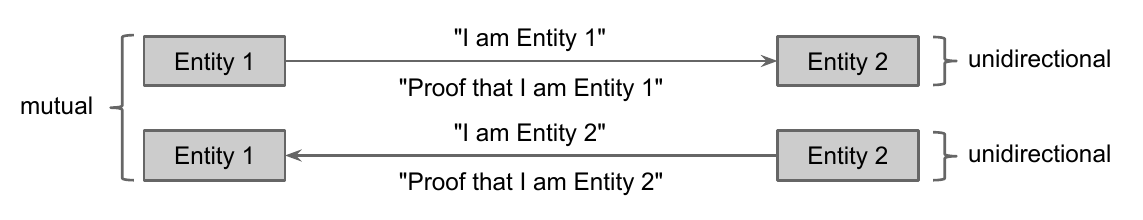
\includegraphics[width=0.9\textwidth]{Images/2Auth.png}
    \caption{Mutual Authentication}
\end{figure}
The entities that enter the process of authentication may be different: i could
have \textbf{human to human} auth, \textbf{human to computer} and 
\textbf{computer to computer}.

To authenticate we need a \textbf{proof of identity}, this may be:
\begin{itemize}
    \item Something the entity \textbf{knows} - passowrd, PIN, handshake
    \item Something the entity \textbf{has} - door key, token
    \item Something the entity \textbf{is} - face, voice, fingerprints
\end{itemize}

\subsection{To-Know Factor}
Passwords and PINs are \textbf{easy to deploy and to implement} with 
\textbf{low implementation costs} (code is "free"): the main problem of 
passwords is that they are easy to be obtained by an attacker. 
\begin{itemize}
    \item \textbf{Guessing} - an attacker can guess a password by identifying similar 
    common patterns between different passwords 
    \item \textbf{Stealing} - a flying note on the office can be always stolen
    \item \textbf{Brute Forcing} - numerous attempts to decode the passwords
\end{itemize}
Also, a data breach made by someone that steals my password for a domain can
be used for accessing with the same keyword to a different domain (mixture of
guessing and stealing)\newline
How can we make the password authentication process is more secure as 
developers and also as users?
\begin{itemize}
    \item \textbf{Change} them continuously
    \item Make them \textbf{long}
    \item Make them \textbf{complex} with special and non-repeatable characters
\end{itemize}
\begin{notice}{Remember}
    Countermeasures are \textbf{costs}: humans are the weakest link in the
    chain of cybersecurity, they hardly remember complex passwords and to 
    force them to write more difficult ones leads to indirect costs.
\end{notice}
A standard problem in cybersecurity is creating a secure communication channel
(such as HTTPS), we will now see how this is possible.

\subsubsection{Secure Exchange}
The game of authentication consists in finding a way to securely share a secret
and in the \textbf{challenge-response scheme} is made possible thanks to 
hashing sent values.
\begin{figure}[H]
    \centering
    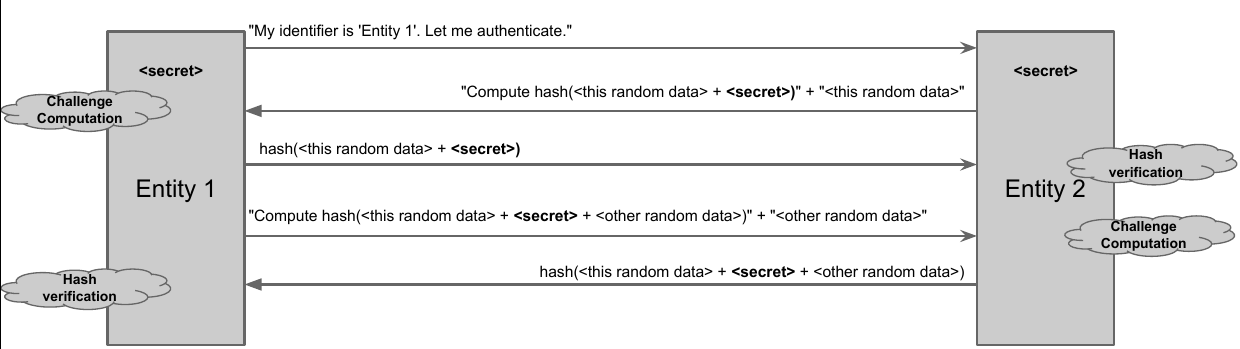
\includegraphics[width=1\textwidth]{Images/3ChallengeResponse.png}
    \caption{Challenge-Response scheme}
\end{figure}
The only problem of this system is that it is enough to breach inside Entity2
to know every secret of every user interfacing with it, meaning that this is not
a feasible solution to implement in reality (see haveibeenpwned).

\subsubsection{Secure Storage}
I need to find a way to "remove" the option of stealing the information, i need
to store my password in a \textbf{hashed way}: when i login, my password gets
hashed, checked (the hashed one, not the true one) and then login happens, only
the hashed version of my password gets saved. If an attacker gets to the 
storage of my machine he will only see my hashed version of the password, that
is \textbf{unusable}.\newline
Now the new problem is \textbf{brute force attacks}, that could try and find 
all passwords that match the hashed result. A solution to those brute force 
attacks is \textbf{salting}: adding a random number stored somewhere else in 
the system to the password and then hash it together.

\subsection{To-Have Factor}
The possession of a key is easy, cheap and comes with a good level of security,
but carries a lot of problems: it's \textbf{hard to deploy} and most importantly
\textbf{hard to share} at the start of the "conversation". There are many 
classic tecnologies that try to cope with those problems:
\begin{itemize}
    \item \textbf{One-Time Password Generators} - user has a device with a 
    counter that is synchronized with the one of the authenticator and changes
    every 30-60 seconds, if communicated counter + key is correct then user is
    authenticated
    \begin{warning}{Synchronization}
        If the device is not kept synchronized overtime then it breaks
    \end{warning}
    \item \textbf{Smart Cards} - the key lies inside a physical integrated 
    circuit and the authentication is done by a challenge-response protocol
    \begin{warning}{Tampering}
        If the device is not tamper proof, then it should not be trusted
    \end{warning}
    \item \textbf{Static OTP Lists} - static tables with codes that corresponds
    to codes saved both by the user and the host (outdated)
    \begin{warning}{Easy to steal}
        A simple look at the physical card and all your codes are gone, a 
        simple listen of some communications between you and the host and at 
        least one code is gone, and so on
    \end{warning}
    \item \textbf{Token OTPs} - the same key logic of OTP generators, but this
    time using software that is embedded and closed
    \begin{warning}{Difficult to defend}
        Since the OPT generator is your phone and since it is a multi-purpose
        device, it is harder to secure and protect (see malicious software)
    \end{warning}
\end{itemize}
There are also a lot of \textbf{scam attacks} and \textbf{impersonating thefts}
linked with physical devices (see the SIM scam).

\subsection{To-Be Factor}
The most common ways to authenticate nowadays are linked to identity as 
\textbf{something we have}, biometric authentication: this has a high level of
security and requires no extra hardware to carry around (we are the key!). 
There are a lot of issues linked to this particular factor: it's \textbf{hard
to deploy safely}, has an \textbf{invasive approach} thanks to its nature, it
\textbf{can be cloned} and also \textbf{changes overtime}